%------------------------------- JPAD: an overview --------------------------------
\chapter{JPAD: an overview}
\label{chap1}

The conceptual and preliminary design phases play a very important role for the development of the future transport aircraft. A computational framework capable of finding an optimal configuration satisfying several basic requirements would be an essential tool for industrial aircraft designers. Such software should be developed around all those basic principles and approaches to aircraft preliminary design well described in several textbooks on the subject. \cite{nicolai2010fundamentals}\cite{roskamAirplane}\cite{torenbeekAAD}

\bigskip
\noindent
A modern preliminary aircraft design tool should be characterized by a certain level of accuracy and reliability, the capability to perform multidisciplinary analyses, and reasonably short computational times. Because of the particular relevance of production costs, noise, emissions, maintenance, and operative costs in the commercial success of a transport aircraft, a modern software framework should be developed with a \gls{MDO} approach in mind. Another important aspect is the user-friendliness of the interface that should allow the user to interact with the design framework in an easy, fast and efficient way. Of the same importance is the possibility to include in the software multiple fidelity analysis methods or to modify and develop new semi-empirical models to achieve better accuracy. It shoul also be possible to export the aircraft configuration geometry (e.g., as a \gls{CAD} model) in one or more standard formats and to execute high-fidelity analyses with external tools (e.g., \gls{CFD} or \gls{FEM} solvers).

\bigskip
\noindent
The present chapter gives an overview of \gls{JPAD}, a Java-based desktop application for aircraft designers. The aim of \gls{JPAD}, which eventually will be released as open-source software, is to provide a library and a set of companion tools based on modern software technology as a support for typical preliminary design studies. The software has been conceived to be used in an industrial environment across conceptual and preliminary design phases. In these phases, a lot of different configurations have to be considered, and so the proposed software relies mostly on semi-empirical analysis methods and is capable to quickly provide results.

%------------------------------- Java choice --------------------------------
\section{Java choice}
\label{sec1.1}

The main challenge in developing from scratch a computational ecosystem to be used by aircraft designers is the choice of the programming language and its related software technology. On the domain modeling side, another challenge is the abstraction of the aircraft, with all its subsystems and subcomponents, as well as the interface with a wide range of analysis tools (related to a number of different disciplines and with different levels of fidelity). So, the programming language has to be chosen according to several considerations. Regarding \gls{JPAD}, Java has been selected for the following reasons: 
%
\begin{itemize}
\item it is widely supported,
\item it promotes the use of open-source libraries (especially for I/O tasks and for complex mathematical operations),
\item there are several \gls{IDE} providing a selection of widely supported \gls{acr:GUI} frameworks and \gls{acr:GUI} visual builders,
\item it supports the object-oriented design pattern and promotes modularity,
\item it naturally allows the development of portable software.
\end{itemize}
%
Java is currently backed by Oracle and by a huge community of developers, and so it is continuously updated. Also, advanced and freely available \gls{IDE}s (such as Eclipse, Netbeans and IntelliJ) allow programmers to streamline and simplify the development process. According to the TIOBE index, in terms of popularity, during the last years the Java language has proven to be the most use among the developers community, as shown in figure \ref{fig:TIOBEIndex}.

\bigskip
\noindent
With Java being a pure object-oriented programming language, it greatly encourages and simplifies modularization. Each module (package) can be programmed quite independently so that it is relatively easy to divide the work among several programmers. This is essential because the amount of classes and calculation needed to abstract, manage, and analyze the entire aircraft is very large. For such a reason, the establishment of common practices and the adherence to fundamental principle of software development (namely, \emph{do not repeat yourself}, \emph{separation of concerns}, \emph{agile software development}) are equally important.

\bigskip
\noindent
The abstraction of the aircraft geometry, its subcomponents (fuselage, lifting surfaces, nacelles, undercarriage, etc.), and their inherent features (weight breakdown, aerodynamic loads, engine deck, etc.) should be effective and general at the same time. This is a typical problem of domain modeling, which has been solved with the object-oriented design pattern naturally provided by the Java language.
%
\begin{figure}[H]
\centering
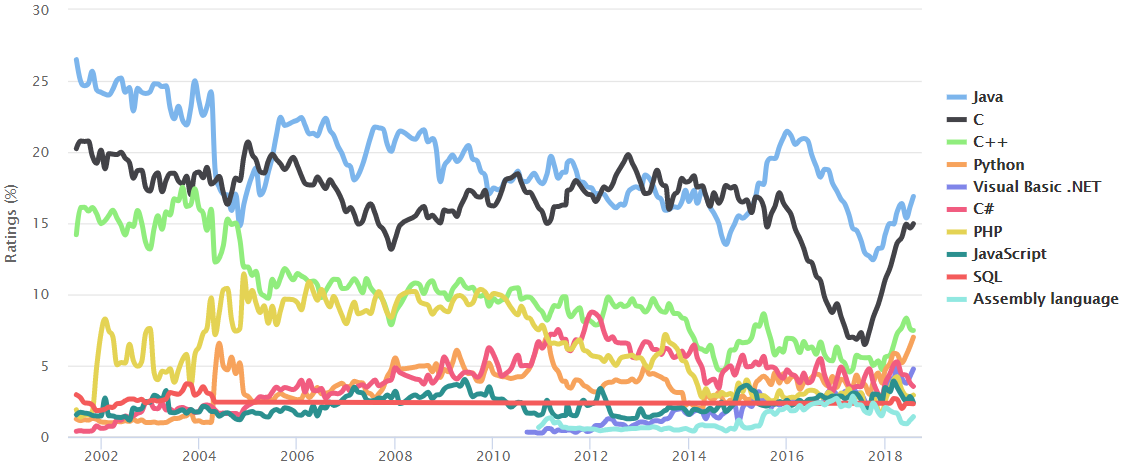
\includegraphics[scale=1.60]{Immagini/Capitolo1/TIOBEIndex}
\caption{TIOBE Programming Community Index (\href{www.tiobe.com}{www.tiobe.com})}
\label{fig:TIOBEIndex}
\end{figure}
%

%------------------------------ Software architecture -----------------------------
\section{Software architecture}
\label{sec1.2}

The following paragraphs deal with the organization of the code. In particular, the first paragraph describes how aircraft data is stored in XML files, while the second one focuses on the packages which constitutes \gls{JPAD}. There are currently six main packages and in the following chapters attention will be particularly focused on two of them: \lstinline[language=Java]!JPADCAD! and \lstinline[language=Java]!JPADCADSandbox!. The last section, instead, gives a brief overview on how and which kind of analyses are performed in \gls{JPAD}.

\subsection{Input files}
As previously mentioned, the input file type for \gls{JPAD} is the XML. In this way, aircraft data, operating conditions, and analyses requirements can be read by the software. XML stands for \emph{eXtensible Markup Language}. It is defined \emph{Markup Language} due to the use of tags that describe the content but, unlike other languages of the same type, the tags created in XML are self explanatory and the user is free to define his own tags, hence the \emph{eXtensible} definition. For this reason documents encoded using the XML format are both human-readable and machine-readable. XML support is provided by many programming languages (including Java) to create and process XML data. Simplicity, portability, platform independence, and usability are some of the key features that have resulted in the increasing popularity of the use of XML based standards. \cite{xmlWiki}

\bigskip
\noindent
More specifically, the XML file format can be summarized by the following concepts:
%
\begin{itemize}
\item tag,
\item attribute,
\item tree structure.
\end{itemize}
%
Each of the above mentioned points is reported in figure \ref{fig:xmlExample}: tags, which are contained between two brackets, are completely personalizable, can be completed by some attributes (such as units of measure) and can be innested, in order to obtain a convenient tree structure suitable for encoding typical data structures.
%
\begin{figure}[H]
\centering
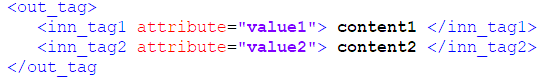
\includegraphics[scale=2.40]{Immagini/Capitolo1/xmlExample}
\caption{A simple XML example}
\label{fig:xmlExample}
\end{figure}
%

\bigskip
\noindent
In order to represent through the use of XML files the typical aircraft data structure, the input file setup designed by the Stanford University for their SUAVE project \cite{SUAVEProject} has been taken into account, deriving from it the folder tree represented in figure \ref{fig:JPADinputfoldertree}. As the figure shows, there's not just one input file storing all the data related to the aircraft. Instead, there's a XML file for each aircraft component and, as shown below, each component can call other XML files (e.g., lifting surfaces XMLs call for airfoil XMLs). The setup of a hierarchy among the XML files helps to reduce dramatically the dimension of each file and makes working with configuration files much easier, especially at high-level. In fact, the user can work fast and simply, assembling custom aircrafts through combination of chosen components XML files. An example of this capability is shown in listing \ref{lst:AircraftXML}, \ref{lst:HTailXML} and \ref{lst:AirfoilXML}. Figure \ref{fig:JPADinputfoldertree} also shows that a similar approach has been followed on the analysis side, splitting analysis XML in multiple files, each one dealing with a specific type of task (see also listing \ref{lst:AnalysesXML}).
%
\begin{figure}[H]
\centering
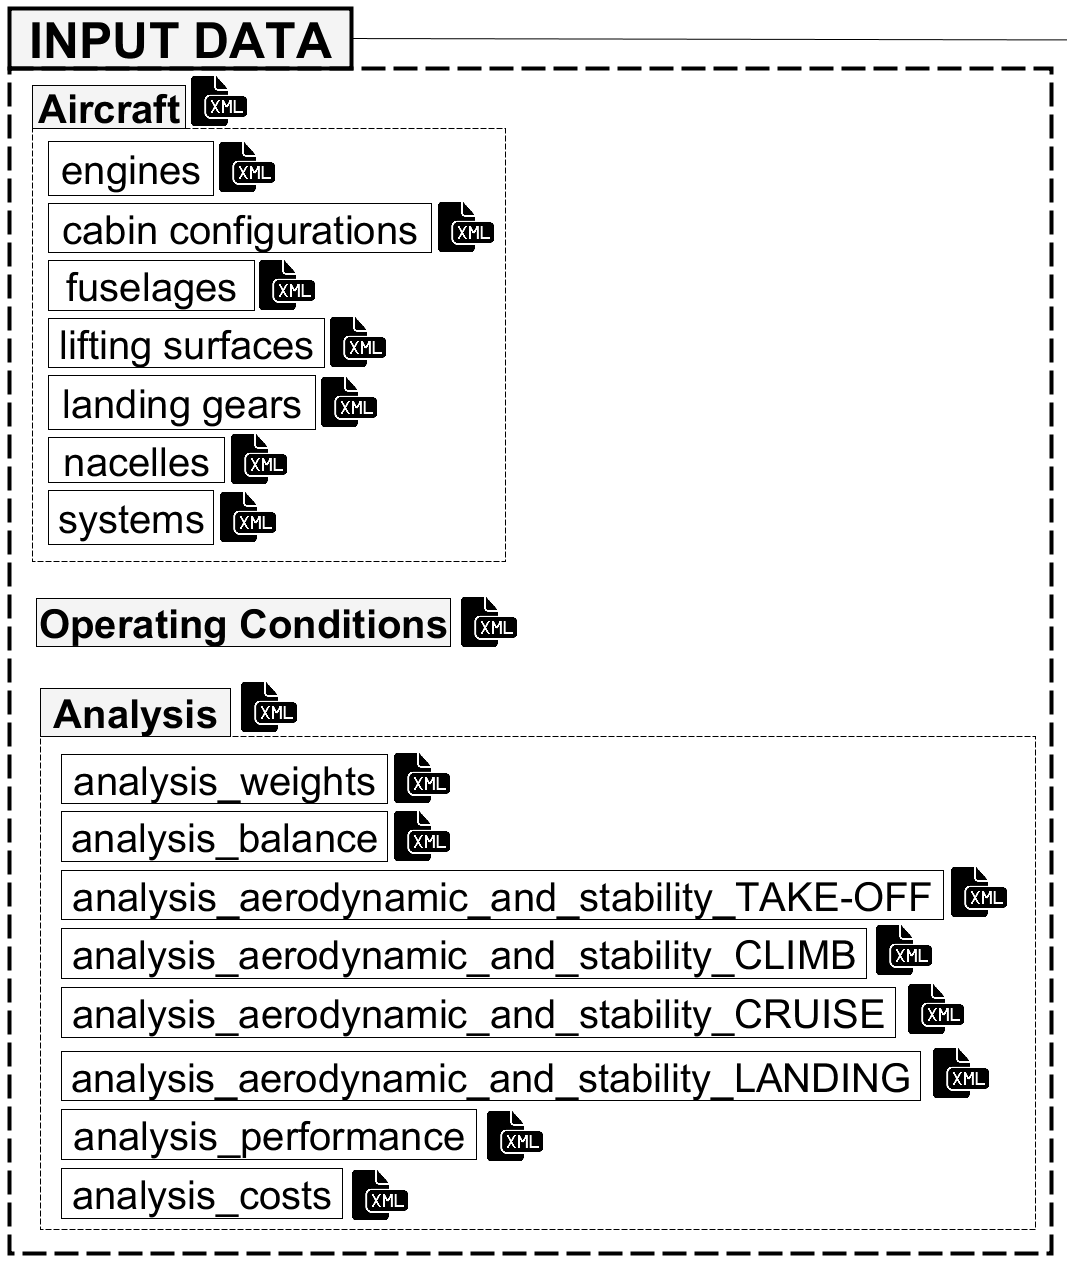
\includegraphics[scale=0.85]{Immagini/Capitolo1/JPADInputData}
\caption{JPAD input folder tree}
\label{fig:JPADinputfoldertree}
\end{figure}
%

\bigskip
\begin{lstlisting}[caption={Example of JPAD aircraft XML file}, captionpos=b, tabsize=6, language=XML, label={lst:AircraftXML}]
<jpad_config>
   <aircraft id="ATR-72" regulations="FAR_25" type="TURBOPROP">
      <lifting_surfaces>
         <wing file="wing_ATR72.xml">
            <position>
               <x unit="m">10.8</x>
               <y unit="m">0.0000</y>
               <z unit="m">1.6</z>
            </position>
            <rigging_angle unit="deg">3.0000</rigging_angle>
         </wing>
         <vertical_tail file="vtail_ATR72.xml">
            <position>
               <x unit="m">21.6</x>
               <y unit="m">0.0000</y>
               <z unit="m">1.3</z>
            </position>
            <rigging_angle unit="deg">0.0000</rigging_angle>
         </vertical_tail>
         <horizontal_tail file="htail_ATR72.xml">
            <position>
               <x unit="m">25.3</x>
               <y unit="m">0.0000</y>
               <z unit="m">5.7374</z>
            </position>
            <rigging_angle unit="deg">1.0000</rigging_angle>
         </horizontal_tail>
      </lifting_surfaces>
      <fuselages>
         <fuselage file="fuselage_ATR72.xml">
            <position>
               <x unit="m">0.0000</x>
               <y unit="m">0.0000</y>
               <z unit="m">0.0000</z>
            </position>
         </fuselage>
      </fuselages>
   </aircraft>
</jpad_config>
\end{lstlisting}

\bigskip
\begin{lstlisting}[caption={Example of JPAD lifting surface XML file}, captionpos=b, tabsize=6, language=XML, label={lst:HTailXML}]
<jpad_config>
   <horizontal_tail id="Horizontal tail" mirrored="true">
      <panels>
         <panel id="ATR72 horizontal tail">
            <span unit="m">3.6548</span>
            <dihedral unit="deg">0.0000</dihedral>
            <sweep_leading_edge unit="deg">13.4400</sweep_leading_edge>
            <inner_section>
               <chord unit="m">2.0440</chord>
               <airfoil file="naca0012.xml"/>
               <geometric_twist>0.000000</geometric_twist>
            </inner_section>
            <outer_section>
               <chord unit="m">1.1652</chord>
               <airfoil file="naca0012.xml"/>
               <geometric_twist unit="deg">0.0000</geometric_twist>
            </outer_section>
         </panel>
      </panels>
      <symmetric_flaps>
         <symmetric_flap id="Elevator" type="PLAIN">
            <inner_station_spanwise_position>0.1</inner_station_spanwise_position>
            <outer_station_spanwise_position>0.9</outer_station_spanwise_position>
            <inner_chord_ratio>0.3000</inner_chord_ratio>
            <outer_chord_ratio>0.3000</outer_chord_ratio>
            <min_deflection unit="deg">-25.0</min_deflection>
            <max_deflection unit="deg">5.0</max_deflection>
         </symmetric_flap>
      </symmetric_flaps>
   </horizontal_tail>
</jpad_config>
\end{lstlisting}

\bigskip
\begin{lstlisting}[caption={Example of JPAD airfoil XML file}, captionpos=b, tabsize=2, language=XML, label={lst:AirfoilXML}]
<jpad_config>
    <airfoil family="NACA_4_Digit" name="NACA0012" type="CONVENTIONAL">
        <geometry>
            <thickness_to_chord_ratio_max>0.1200</thickness_to_chord_ratio_max>
            <radius_leading_edge_norm unit="m">0.0158</radius_leading_edge_norm>
            <x_coordinates>[...]</x_coordinates>
            <z_coordinates>[...]</z_coordinates>
        </geometry>
        <aerodynamics>
            <alpha_zero_lift unit="deg">0.0000</alpha_zero_lift>
            <alpha_end_linear_trait unit="deg">11.0000</alpha_end_linear_trait>
            <alpha_stall unit="deg">20.1000</alpha_stall>
            <Cl_alpha_linear_trait unit="1/rad">6.9200</Cl_alpha_linear_trait>
            <Cl_at_alpha_zero>0.000000</Cl_at_alpha_zero>
            <Cl_end_linear_trait>1.2300</Cl_end_linear_trait>
            <Cl_max>1.8600</Cl_max>
            <Cd_min>0.005500</Cd_min>
            <Cl_at_Cdmin>0.000000</Cl_at_Cdmin>
            <laminar_bucket_semi_extension>0.000000</laminar_bucket_semi_extension>
            <laminar_bucket_depth>0.000000</laminar_bucket_depth>
            <K_factor_drag_polar>0.003500</K_factor_drag_polar>
            <Cm_alpha_quarter_chord unit="1/deg">0.0000</Cm_alpha_quarter_chord>
            <Cm_ac>0.000000</Cm_ac>
            <Cm_ac_at_stall>-0.090000</Cm_ac_at_stall>
            <x_ac_normalized>0.2500</x_ac_normalized>
            <mach_critical>0.7340</mach_critical>
            <x_transition_upper>0.1200</x_transition_upper>
            <x_transition_lower>0.1200</x_transition_lower>
        </aerodynamics>
    </airfoil>
</jpad_config>
\end{lstlisting}

\subsection{Libraries}
\gls{JPAD} is currently made of six main packages, each one of them dealing with specific tasks. Moreover, each package can contain several sub-packages (organized in classes and utilities) pertinent to more specialized assignments. This kind of organization, called modularity, helps in terms of code mainteinance: part of the system can be updated in case of issues without a need to make large-scale changes. Besides, modularity makes working with the code much easier in an ever changing team.

\bigskip
\noindent
The six packages that constitutes \gls{JPAD} are: \lstinline[language=Java]!JPADCore! (actually, \lstinline[language=Java]!JPADCore_v2! due to the intense changes occurred during the last months), \lstinline[language=Java]!JPADConfigs!, \lstinline[language=Java]!JPADCommander!, \lstinline[language=Java]!JPADCAD!, \lstinline[language=Java]!JPADSandBox! (actually, \lstinline[language=Java]!JPADSandBox_v2!), and \lstinline[language=Java]!JPADCADSandBox!. The next sections describe each package individually, summarizing the characteristics and the tasks of each one of them.

\subsubsection{\texttt{JPADCore}}
\lstinline[language=Java]!JPADCore!, as the name suggests, is \gls{JPAD} main package. It currently contains the following sub-packages.
%
\begin{itemize}
\item \lstinline[language=Java]!aircraft!, which contains sub-packages dedicated to aircraft components (fuselage, lifting surfaces, nacelles, power plant, cabin configuration) and classes managing landing gears and systems mounted on board. As previously mentioned for the input XML structure side, the lifting surfaces package also contains the classes managing the airfoils.
\item \lstinline[language=Java]!analyses!, which contains the managers for five types of analysis that can be performed on aircrafts: weights, balance, aerodynamics and stability, performance, and costs. Additionally, \lstinline[language=Java]!analyses! also contains sub-packages (one for each of the before mentioned aircraft components) enclosing component's manager classes for weigths, balance and aerodynamic calculation. Finally, classes managing the operating conditions are stored in this package too.
\item \lstinline[language=Java]!calculators!, actually containing all the methods and the formulas needed to perform all the previously mentioned analyses.
\item \lstinline[language=Java]!database!, containing the classes used in order to read data from HDF files (reader can refer to \cite{HDFWiki} for more information about). In particular, these classes manage the data reading process from aerodynamics and engine databases.
\item \lstinline[language=Java]!standaloneutils!, which encloses several utility classes, i.e., classes containing methods that can be accessed in a static way. These utilities cover the most various needings, from Standard Atmoshere properties calculation to XML file reading.
\item \lstinline[language=Java]!writers!, finally, enclosing classes useful in order to store results.
\end{itemize}
%

\subsubsection{\texttt{JPADConfigs}}
\lstinline[language=Java]!JPADConfigs! is the package containing all the enumeration classes used in \gls{JPAD}. In computer programming, enumerations consist of a set of named values. The enumerator names are usually identifiers that behave as constants in the language. In the Java programming language, enumeration types are defined using the \lstinline[language=Java]!enum! keyword; because values assumed by enumeration type variables are constant, the names of an \lstinline[language=Java]!enum! type fields are in uppercase letters. \cite{JavaEnum}

\bigskip
\noindent
Like the \lstinline[language=Java]!standaloneutils! classes, enumerations contained in \lstinline[language=Java]!JPADConfigs! cover very different fields: some such as \lstinline[language=Java]!ComponentEnum! and \lstinline[language=Java]!AirplaneType! regard the aircraft and its characteristics, while others, such as \lstinline[language=Java]!MethodEnum! and \lstinline[language=Java]!AnalysisTypeEnum!, deal with the analyses.

\subsubsection{\texttt{JPADCommander}}
\lstinline[language=Java]!JPADCommander! contains the classes which allow the \gls{JPAD} \gls{acr:GUI} (simply called JPADCommander in the rest of the paragraph) to work. 

\bigskip
\noindent
\gls{JPAD} comes with a simple yet very intuitive \gls{acr:GUI}. In order to simplify the management of all the operations required for the definition of the aircraft parametric model and its analysis, JPADCommander guides the user through a path which starts with the definition of the working folders and ends with the management and visualization of the output. In particular, JPADCommander interfaces with the user by means of four main windows. The first one is a configuration window, through which the user defines:
%
\begin{itemize}
\item working directory,
\item input directory,
\item output directory,
\item database directory.
\end{itemize}
%
The second screen gives the user the possibiity to choose between \emph{Input}, \emph{Analysis} and \emph{Results}. As soon as the user has defined the previously mentioned folders, the only option available is the one regarding the input, with the analysis button becoming available just after the input phase has been performed. The same happens for the results button, which becomes clickable after the user has performed the analysis phase. The third screen, the one regarding the Input Manager, is shown in figure \ref{fig:GUIInputManager}. Here, the user has three possibilities:
%
\begin{itemize}
\item loading a default aircraft,
\item importing aircraft data from file,
\item generating a new aircraft filling in all the fields in the Input Manager screen.
\end{itemize}
%
Figure \ref{fig:GUIInputManager} also shows that the Input Manager screen has several additional pages, dedicated to each of the aircraft components mentioned in the input file section. After completing the input phase, clicking the \emph{Home} button the user will have access to the Analysis Manager screen, which is shown in figure \ref{fig:GUIAnalysisManager}. In this module, the user can define which analyses he wants to perform. As for the Input Manager, also in this case the user has the possibility to load a previously saved analysis or fill in the available fields. Finally, as soon as the analyses have been performed, results become available from the main screen.
%
\begin{figure}[H]
\centering
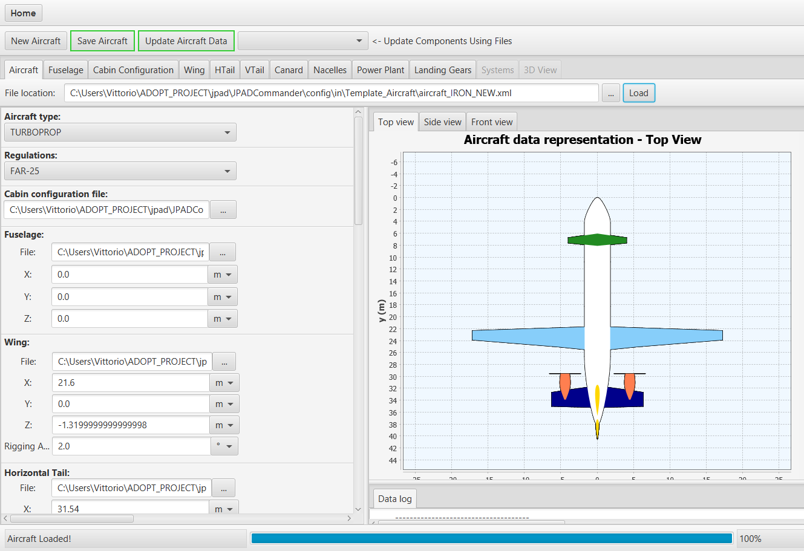
\includegraphics[scale=2.0]{Immagini/Capitolo1/AircraftInputManager}
\caption{JPADCommander Aircraft Input Manager screen}
\label{fig:GUIInputManager}
\end{figure}
%
\begin{figure}[H]
\centering
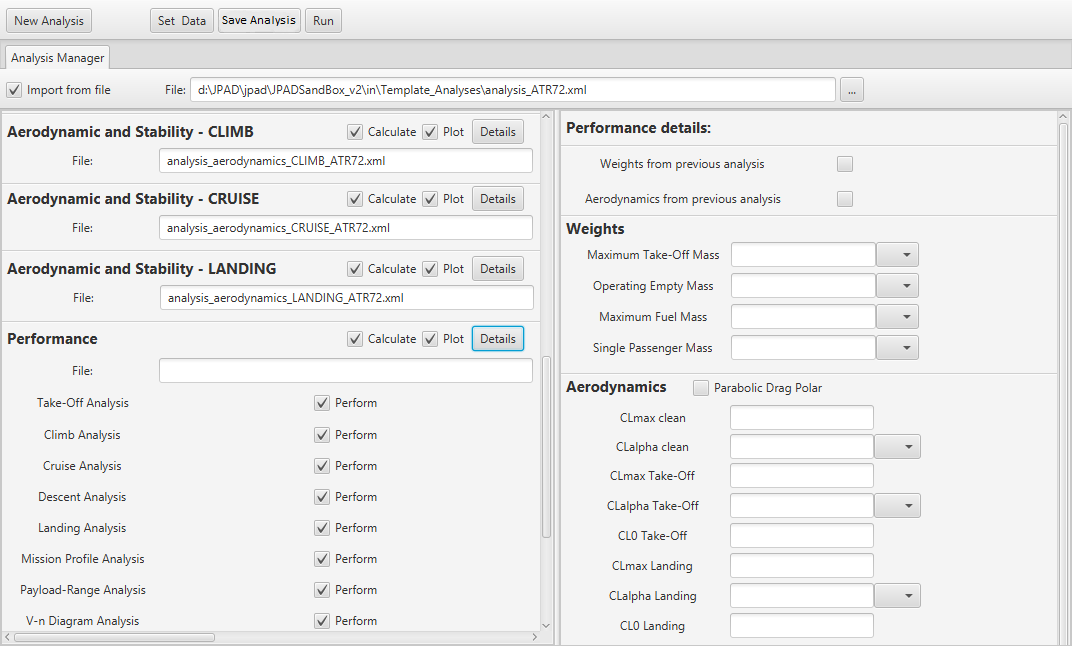
\includegraphics[scale=1.5]{Immagini/Capitolo1/AnalysisManagerGUI}
\caption{JPADCommander Analysis Manager screen}
\label{fig:GUIAnalysisManager}
\end{figure}
%

\subsubsection{\texttt{JPADSandBox}}
This package contains all the test classes, i.e., classes (mostly containing main methods) used in order to test new methods or functionalities, before adding them to \gls{JPAD} main libraries. It encloses several packages, one for each developer, in which individual tests can be written and performed. Besides, it also contains the folders in which template aircraft and analysis XMLs are stored.

\subsubsection{\texttt{JPADCAD} - \texttt{JPADCADSandBox}}
Generating \gls{CAD} models can be an important achievement for a software such as \gls{JPAD} for several reasons.
%
\begin{itemize}
\item It gives an immediate feedback about the data provided to the application: in case of mistakes, the \gls{CAD} model helps detecting them almost immediately.
\item It allows the user to run a \gls{CFD} analysis using an external tool. In fact, \gls{JPAD} generated \gls{CAD} models are ready to be meshed without any further adjustment.
\item It provides an accurate estimate of the wet surface of each component.
\end{itemize}
%
\lstinline[language=Java]!JPADCAD! and \lstinline[language=Java]!JPADCADSandbox! are the packages which currently contain all the classes and utility classes necessary to the creation of geometric and topological entities. Shapes (i.e., basic topological entities) can be exported into various file formats (e.g., STEP or IGES) and opened in any desired \gls{CAD} software. Generating the most various shapes is made possible by the use of the \gls{OCCT} classes, which are actually written in C++, but can be used in \gls{JPAD} thanks to the \gls{OCCT} Java Wrapper, a tool which allows the use of \gls{OCCT} classes from within Java applications. The static methods which actually perform the translation from the aircraft geometric data (stored, as previously mentioned, in the XML file format) to CAD file format currently reside in \lstinline[language=Java]!AircraftUtils!, a \lstinline[language=Java]!JPADCADSandbox! utility class. The same package also contains all the tests performed for this thesis work.

\subsection{Analyses}
\label{sec1.3}

The main purpose of \gls{JPAD} is to perform different analyses and to provide the data necessary for the comparison of different aircraft or different configurations of the same aircraft. The previously described XML structure easily allows this. Besides, the same hierarchical structure has been replicated for the analyses, as reported in listing \ref{lst:AnalysesXML}, giving the user the possibility to perform a complete analysis (i.e., executing all the analyses contained in \lstinline[language=Java]!JPADCore!), or specific ones, combining different analysis files. This allows an easier evaluation of a generic cost function during optimization tasks, resulting in a reduced amount of computational costs required for this kind of operations.

\bigskip
\begin{lstlisting}[caption={JPAD analyses XML file, not needed analyses are commented}, captionpos=b, tabsize=6, language=XML, label={lst:AnalysesXML}]
<jpad_config>
    <!-- Input data, shared across analysis tasks -->
    <global_data>
        <positive_limit_load_factor>2.5</positive_limit_load_factor>
		<negative_limit_load_factor>-1.0</negative_limit_load_factor>
    </global_data>
    <!-- Required analysis tasks - comment the tag of the analysis if not needed -->
    <analyses id="ATR-72 analysis" iterative_loop="FALSE">
		<weights 
            file="analysis_weights_ATR72.xml" 
			plot="TRUE"
			create_CSV="TRUE"
            method_fuselage=""
            method_wing=""
            method_htail=""
            method_vtail=""
			method_canard=""
			method_nacelles=""
			method_power_plant=""
			method_landing_gears=""
			method_APU=""
			method_air_conditioning_and_anti_icing=""
			method_instruments_and_navigation_system=""
			method_hydraulic_and_pneumatic_systems=""			
			method_electrical_systems=""
			method_furnishings_and_equipments=""
			method_control_surfaces=""
            />
		<balance 
			file="analysis_balance_ATR72.xml"
			plot="TRUE"
			create_CSV="TRUE"
            method_fuselage=""
            method_wing=""
            method_htail=""
            method_vtail=""
			method_canard=""
			method_nacelles=""
			method_power_plant=""
			method_landing_gears=""
		/>
		<!--
		<aerodynamic_and_stability
			plot="FALSE"
			create_CSV="FALSE"
			take_off_condition="TRUE"
			file_take_off_condition="analysis_aerodynamics_ATR72_takeoff.xml"
			climb_condition="TRUE"
			file_climb_condition="analysis_aerodynamics_ATR72_climb.xml"
			cruise_condition="TRUE"
			file_cruise_condition="analysis_aerodynamics_ATR72_cruise.xml"
			landing_condition="TRUE"
			file_landing_condition="analysis_aerodynamics_ATR72_landing.xml"
		/>
		<performance 
			file="analysis_performance_ATR72.xml"
			plot="FALSE"
			create_CSV="FALSE"
			take_off="FALSE"
			climb="FALSE"
			cruise="FALSE"
			descent="FALSE"
			landing="FALSE"
			payload_range="FALSE"
			V_n_diagram="FALSE"
			mission_profile="TRUE"
		/>
		<costs 
			file="analysis_costs_ATR72.xml"
			plot="FALSE"
			create_CSV="FALSE"
			doc_capital="TRUE"
			doc_capital_method="AEA"
			doc_crew="TRUE"
			doc_crew_method="AEA"
			doc_fuel="TRUE"
			doc_fuel_method="AEA"
			doc_charges="TRUE"
			doc_charges_method="ILR_AACHEN"
			doc_maintenance="TRUE"
			doc_maintenance_method="ATA"
		/> 
		-->
    </analyses>
</jpad_config>
\end{lstlisting}

\bigskip
\noindent
\gls{JPAD} currently allows five types of analysis.
%
\begin{itemize}
\item Weights analysis: estimates the aircraft weight breakdown starting from a first guess maximum take-off weight and specific mission requirements. In particular, it evaluates each aircraft component mass using well-known semi-empirical methods.
\item Balance analysis: estimates the centre of gravity position related to each weight condition and draws the balance diagram.
\item Aerodynamics and Stability analysis: the aerodynamics module estimates all the aerodynamic characteristics in terms of lift, drag and moment coefficients, at different operating conditons and for each aircraft component (wing, tails, fuselage, and nacelles); whereas the stability module reports data concerning the aircraft static stability.
\item Performance analysis: evaluates aircraft most important performances, such as payload-range diagram, mission profile, cruise flight envelope, ground performance, climb performance, and cruise grid chart.
\item Costs analysis: estimates the \gls{DOC} breakdown.
\end{itemize}
%
In addition to multidisciplinary analyses, \gls{JPAD} is also able to perform parametric studies and \gls{MDO}. In both cases it is possible to define a set of parameters to be varied, typically geometric, and the input manager will provide for the generation of all the test aircrafts thanks to the combination of different files for the individual components. Once all the required configurations are ready, it will be possible to choose whether to carry out a parametric study or an optimization. It will be necessary to define one or more objectives to be monitored and one or more constraints to be respected; the latter can be selected from a dedicated list. Once all the parameters have been defined, \gls{JPAD} will launch all the analyses necessary for the evaluation of the objectives and the required constraints, with the possibility of exploiting serial or parallel analyses (i.e., executed on more threads) in order to reduce calculation times. Once all the required calculation have been completed, one or more response surfaces will be obtained which, on the one hand, constitute the output of the parametric study, while on the other they can be used as input for optimization (figure \ref{fig:JPADParametricStudy}). 
%
\begin{figure}[htbp]
\centering
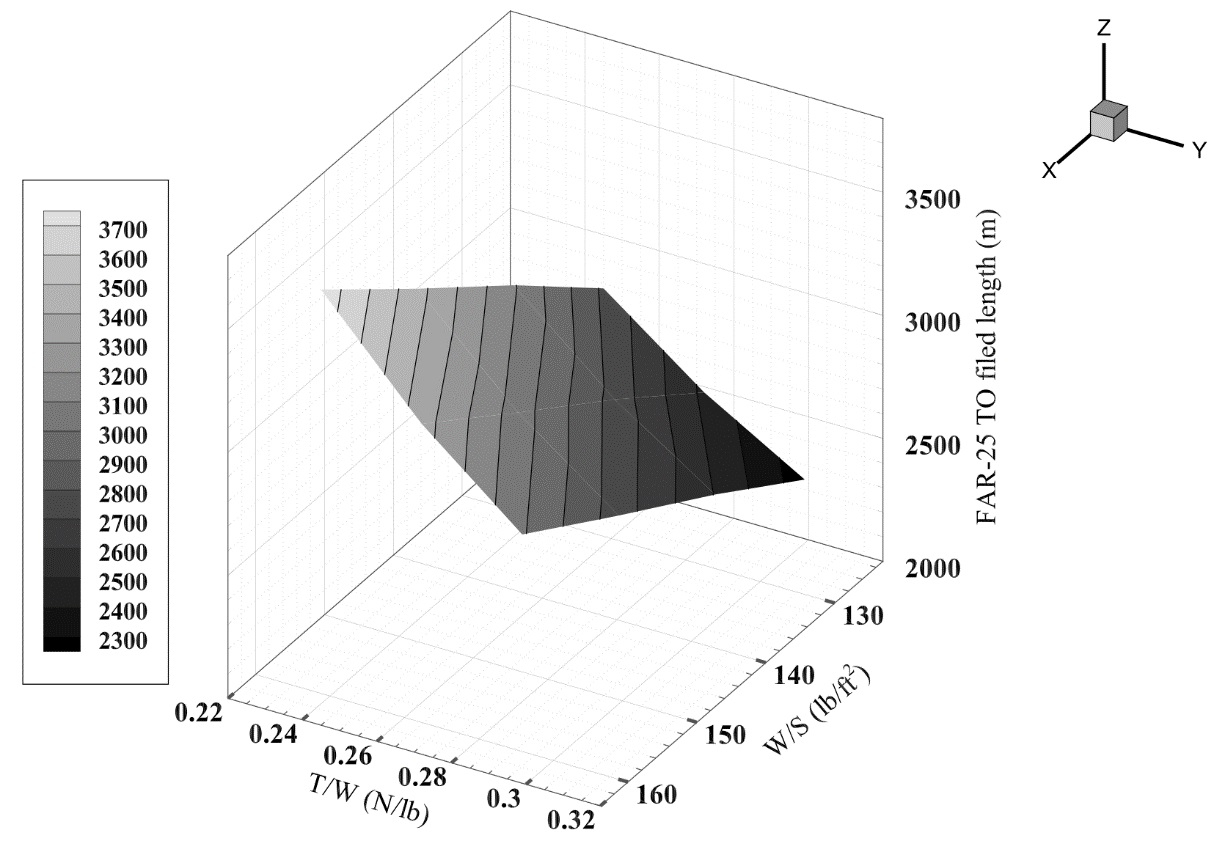
\includegraphics[height=0.27\textheight]{Immagini/Capitolo1/JPADParametricStudy}
\caption{Example of parametric study performed in JPAD on a Boeing B747-100B}
\label{fig:JPADParametricStudy}
\end{figure}
%

\bigskip
\noindent
Figure \ref{fig:JPADFlowchart} shows JPAD typical flowchart, summarizing the concepts expressed in the previous paragraphs. In particular, it clearly makes a distinction between the input (aircraft and analysis data) and the core (the analysis itself).
%
\begin{figure}[htbp]
\centering
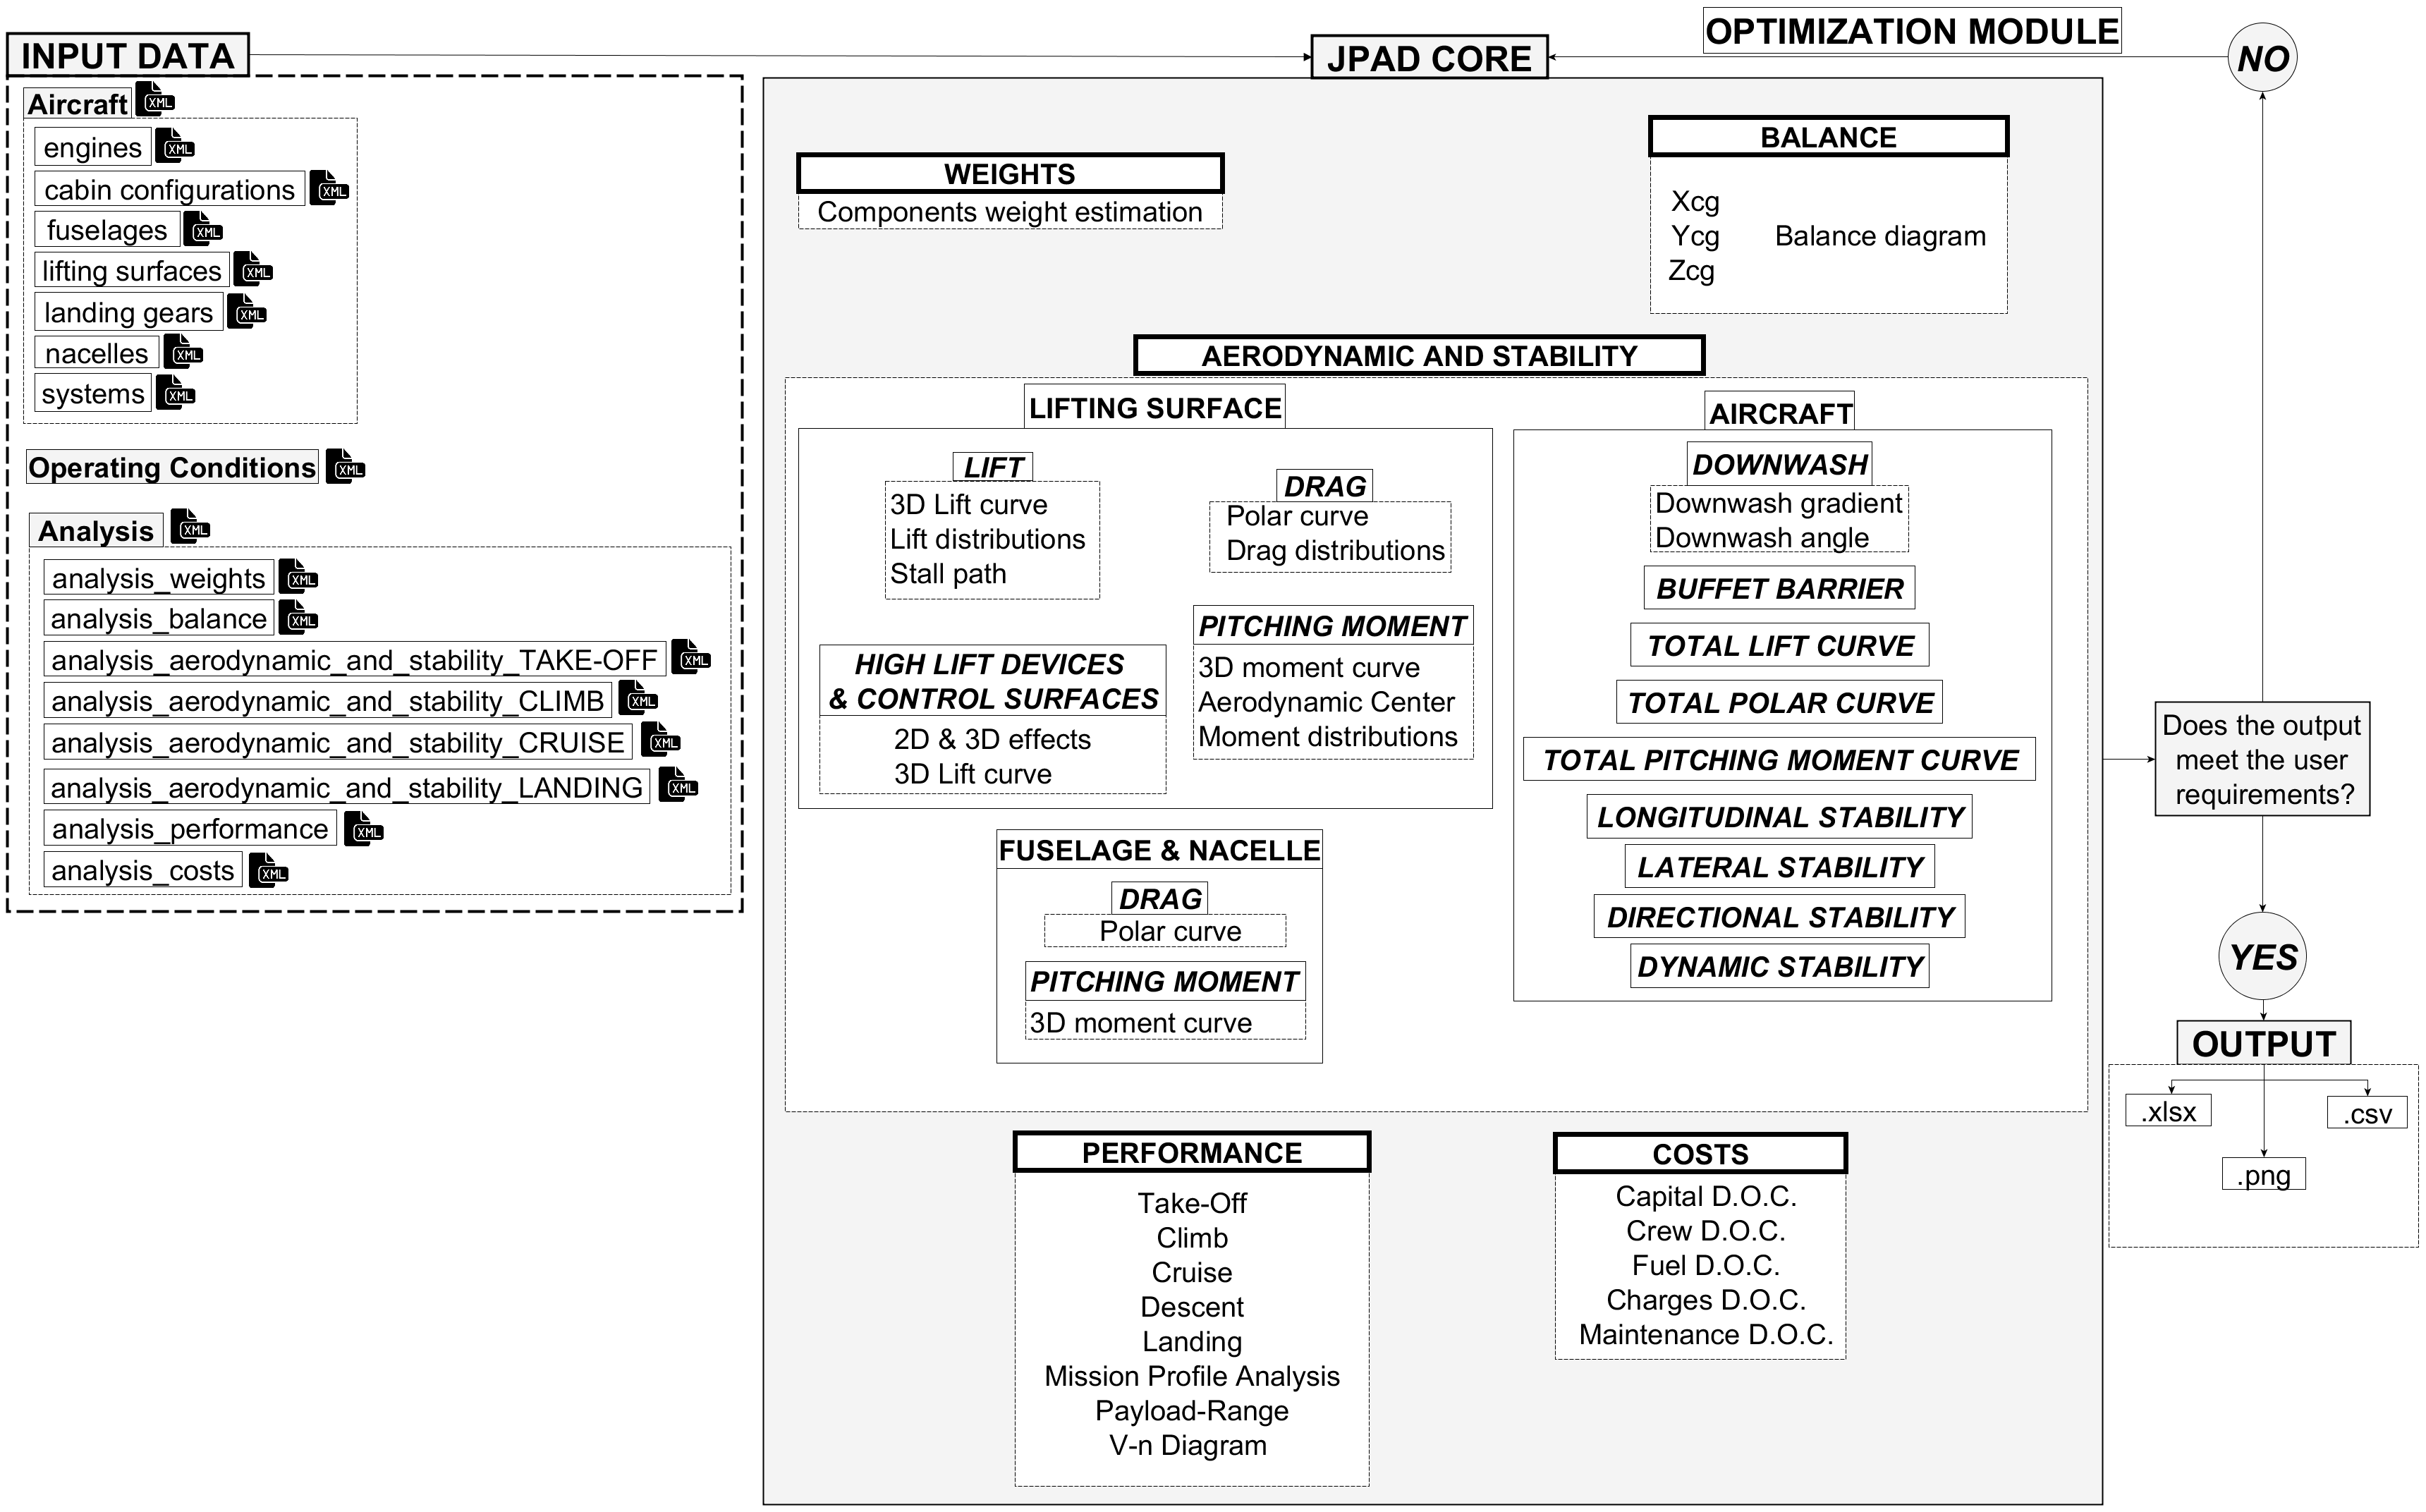
\includegraphics[height=0.36\textheight]{Immagini/Capitolo1/JPADFlowchart}
\caption{JPAD flowchart}
\label{fig:JPADFlowchart}
\end{figure}
%

